%----------------------------------------------------------------------------------------
%	PACKAGES AND DOCUMENT CONFIGURATIONS
%----------------------------------------------------------------------------------------
\documentclass[11pt]{article}

\usepackage{hyperref}
\usepackage{caption}
\usepackage{xcolor}
\usepackage{graphicx} % Required for the inclusion of images
\usepackage{amsmath} % Required for some math elements
\usepackage[margin=24mm]{geometry}
\usepackage{courier}
\usepackage{listings}
\usepackage{graphicx}
\usepackage{subcaption}

\lstset{basicstyle=\footnotesize\ttfamily,breaklines=true}
\captionsetup[figure]{font=small}

\addtolength{\topmargin}{-12mm}
\addtolength{\textheight}{12mm}

\setlength\parindent{0pt} % Removes all indentation from paragraphs
\renewcommand{\labelenumi}{\alph{enumi}.} % Make numbering in the enumerate environment by letter rather than number (e.g. section 6)

\definecolor{mygreen}{RGB}{28,172,0} % color values Red, Green, Blue
\definecolor{mylilas}{RGB}{170,55,241}

\lstset{
		language=Matlab,
    %basicstyle=\color{red},
    breaklines=true,
    %morekeywords={matlab2tikz},
    keywordstyle=\color{blue},
    morekeywords=[2]{1},
		keywordstyle=[2]{\color{black}},
    identifierstyle=\color{black},%
    stringstyle=\color{mylilas},
    commentstyle=\color{mygreen},%
    showstringspaces=false, %without this there will be a symbol in the places where there is a space
    numbers=left,%
    numberstyle={\tiny \color{black}},% size of the numbers
    numbersep=9pt, % this defines how far the numbers are from the text
    emph=[1]{for,end,break},
		emphstyle=[1]\color{red} %some words to emphasise
    %emph=[2]{word1,word2},
		%emphstyle=[2]{style},
}
%----------------------------------------------------------------------------------------
%	DOCUMENT INFORMATION
%----------------------------------------------------------------------------------------

\title{ECEN 220 \\ Lab Report 5 : Upsampling}
\author{Daniel Eisen : 300447549}
\date{\today}

\begin{document}
	\maketitle

\section{Sampling and Zero Padding}
\begin{figure}[h]
	\centering
	\begin{subfigure}[b]{.4\linewidth}
	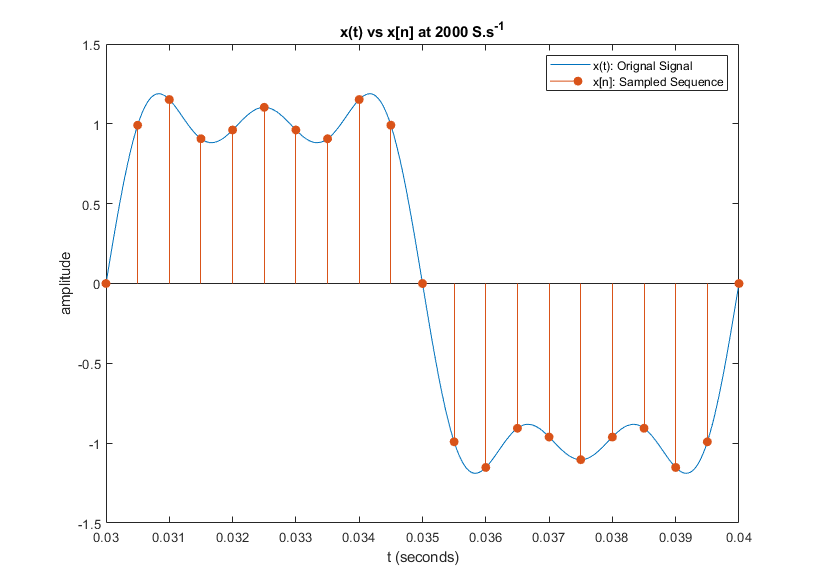
\includegraphics[width=\linewidth]{fig1}
	\caption{signal vs sampled}
	\end{subfigure}
	\begin{subfigure}[b]{.4\linewidth}
	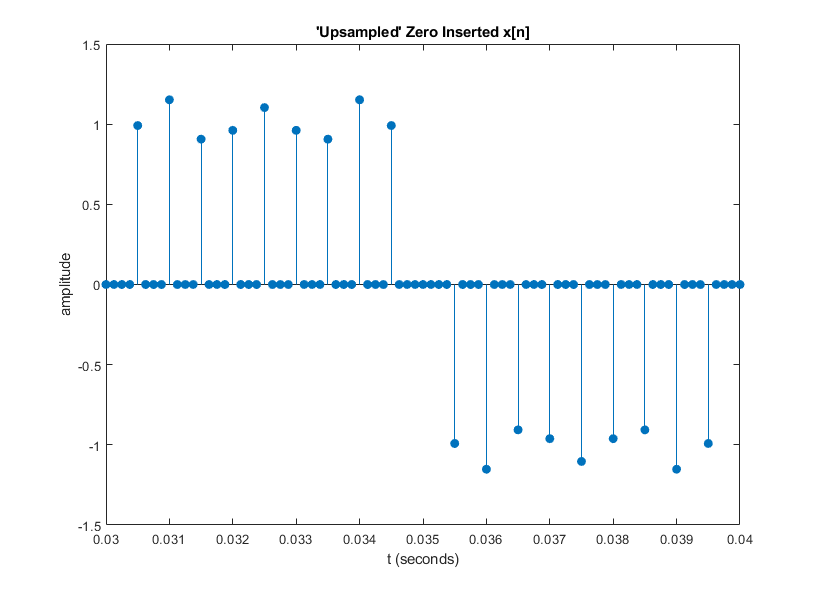
\includegraphics[width=\linewidth]{fig2}
	\caption{Zero Padded}
	\end{subfigure}
\end{figure}

Step one is to sample a CT signal, in this case x(t) is shown in figure 1 to be sampled at 2000 samples a second.
To begin up sampling, the sequence x[n] is zero padded to create a sequence at 8000 samples a second, shown figure 2.

\section{Filter Response Generation}
\begin{figure}[!h]
	\centering
	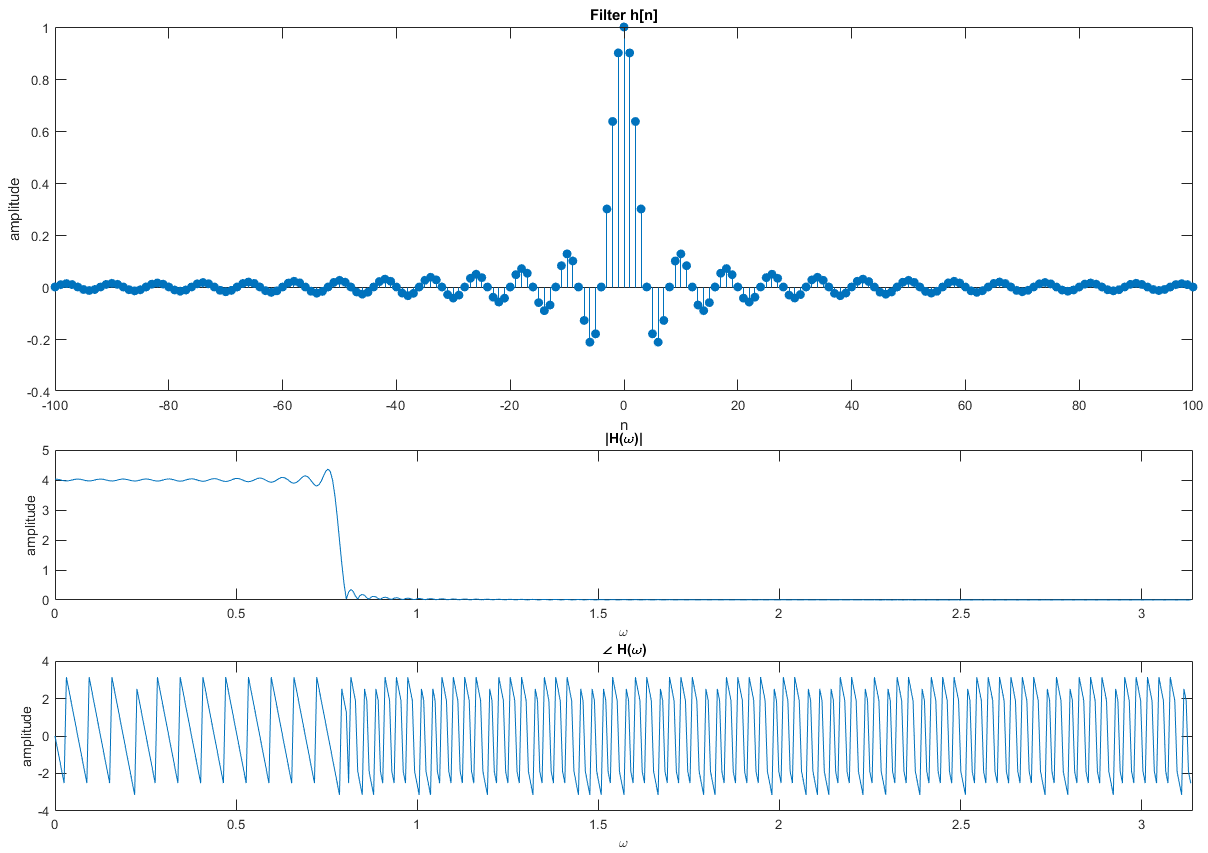
\includegraphics[width=0.5\textwidth]{fig3}
	\caption{Filter and frequency components}
\end{figure}

A sinc is generated for use in low=pass filtering the zero padded sequence for up sampling. The magnitude plot shows the band of allowed frequencies.

\newpage
\section{Low Pass Filtering}

\begin{figure}[!h]
	\centering
	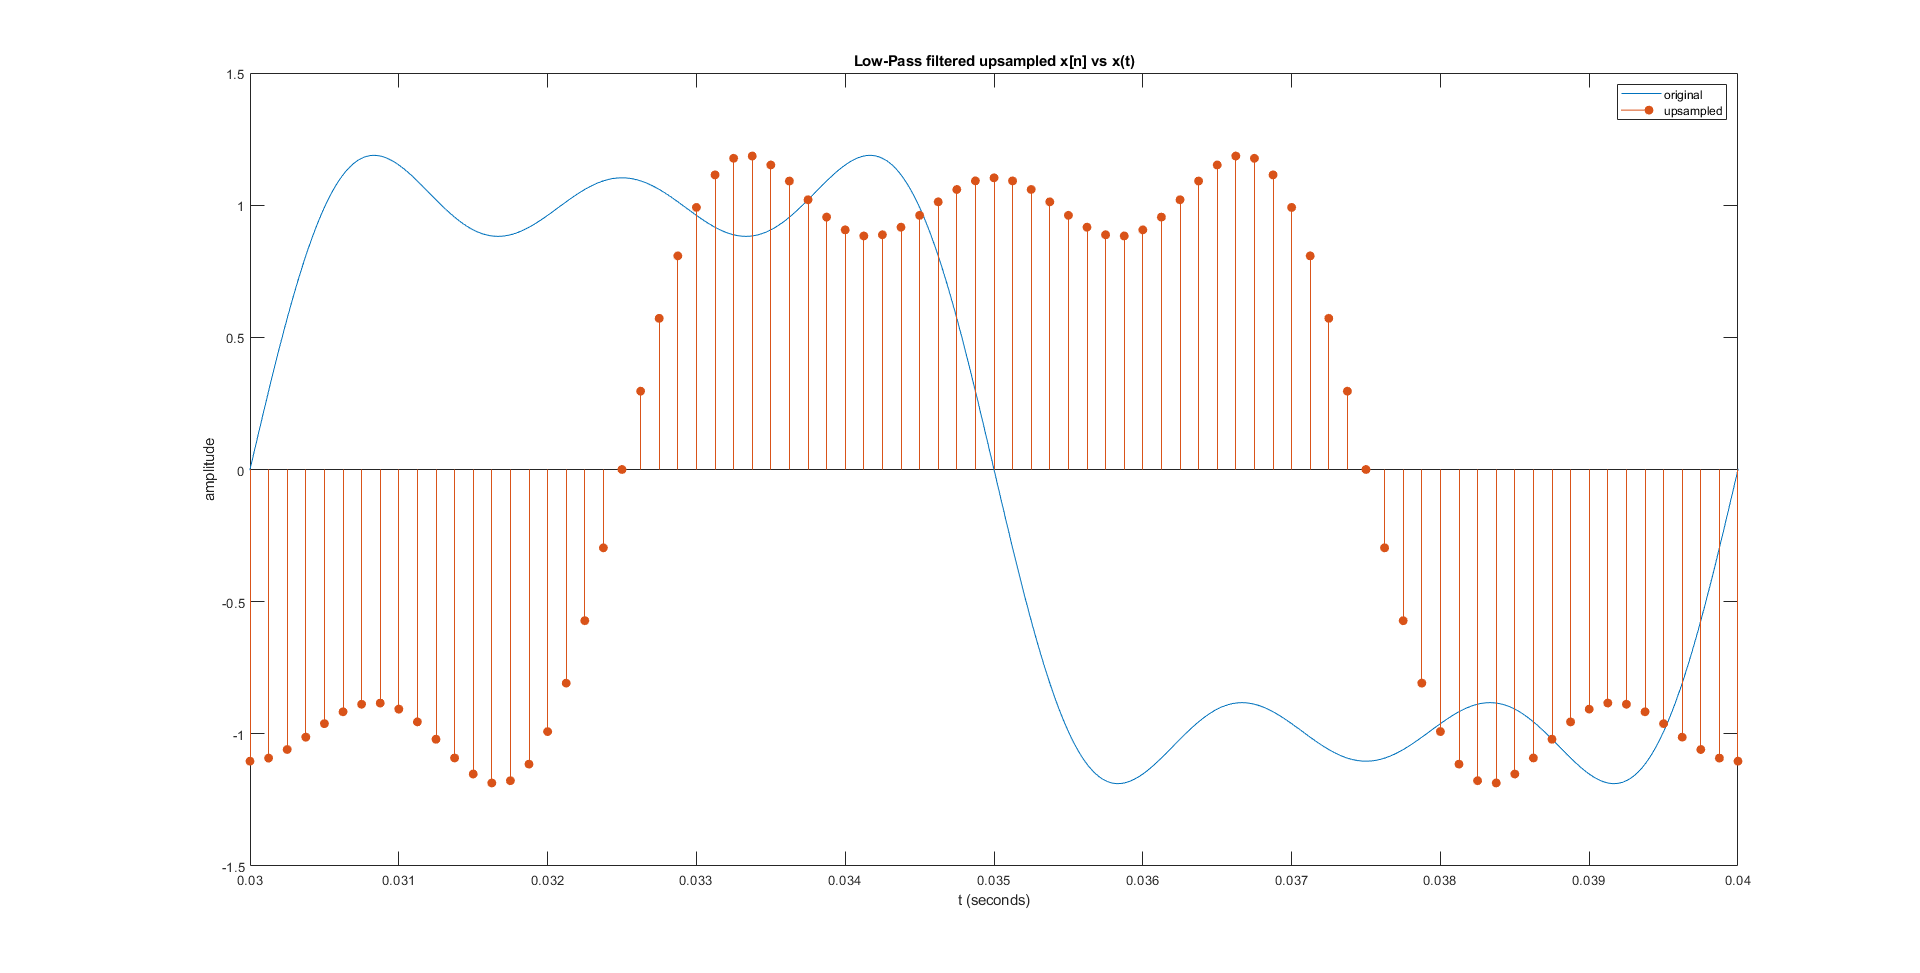
\includegraphics[width=0.8\textwidth]{fig4}
	\caption{Filtered and Reconstructed signal and original signal}
\end{figure}

Upon filtering, figure 3 shows an up sampled sequence that appears to be accurate in form to the original signal, it is however delayed by the length of the filter, so does not match in phase.
\section{Delay Reconstruction}

\begin{figure}[!h]
	\centering
	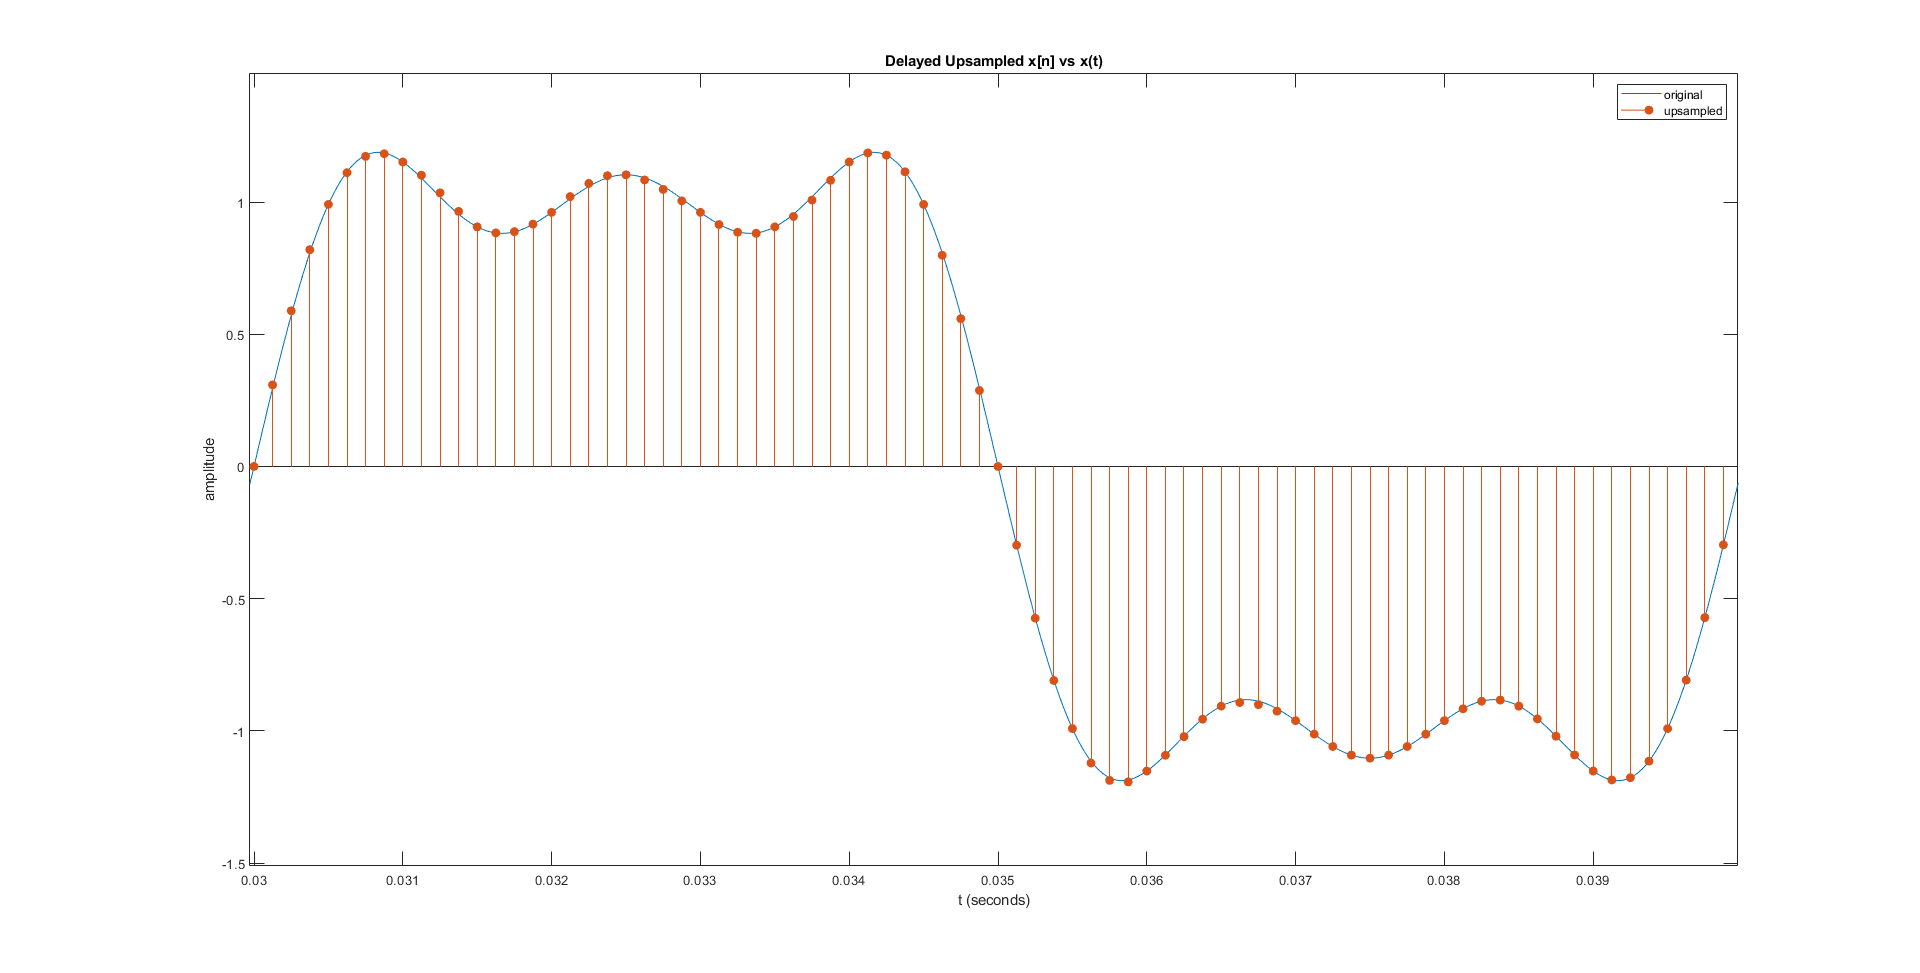
\includegraphics[width=0.8\textwidth]{fig5}
	\caption{Filtered and Reconstructed signal and original signal}
\end{figure}

Figure 5 shows, that upon delaying the sequence by a further filter length, the overlaid signal and sequence are shown to be very close in form, so the original samples have been successfully up sampled.

\newpage
\section{Delaying Effect of Filtering}
\begin{figure}[!h]
	\centering
	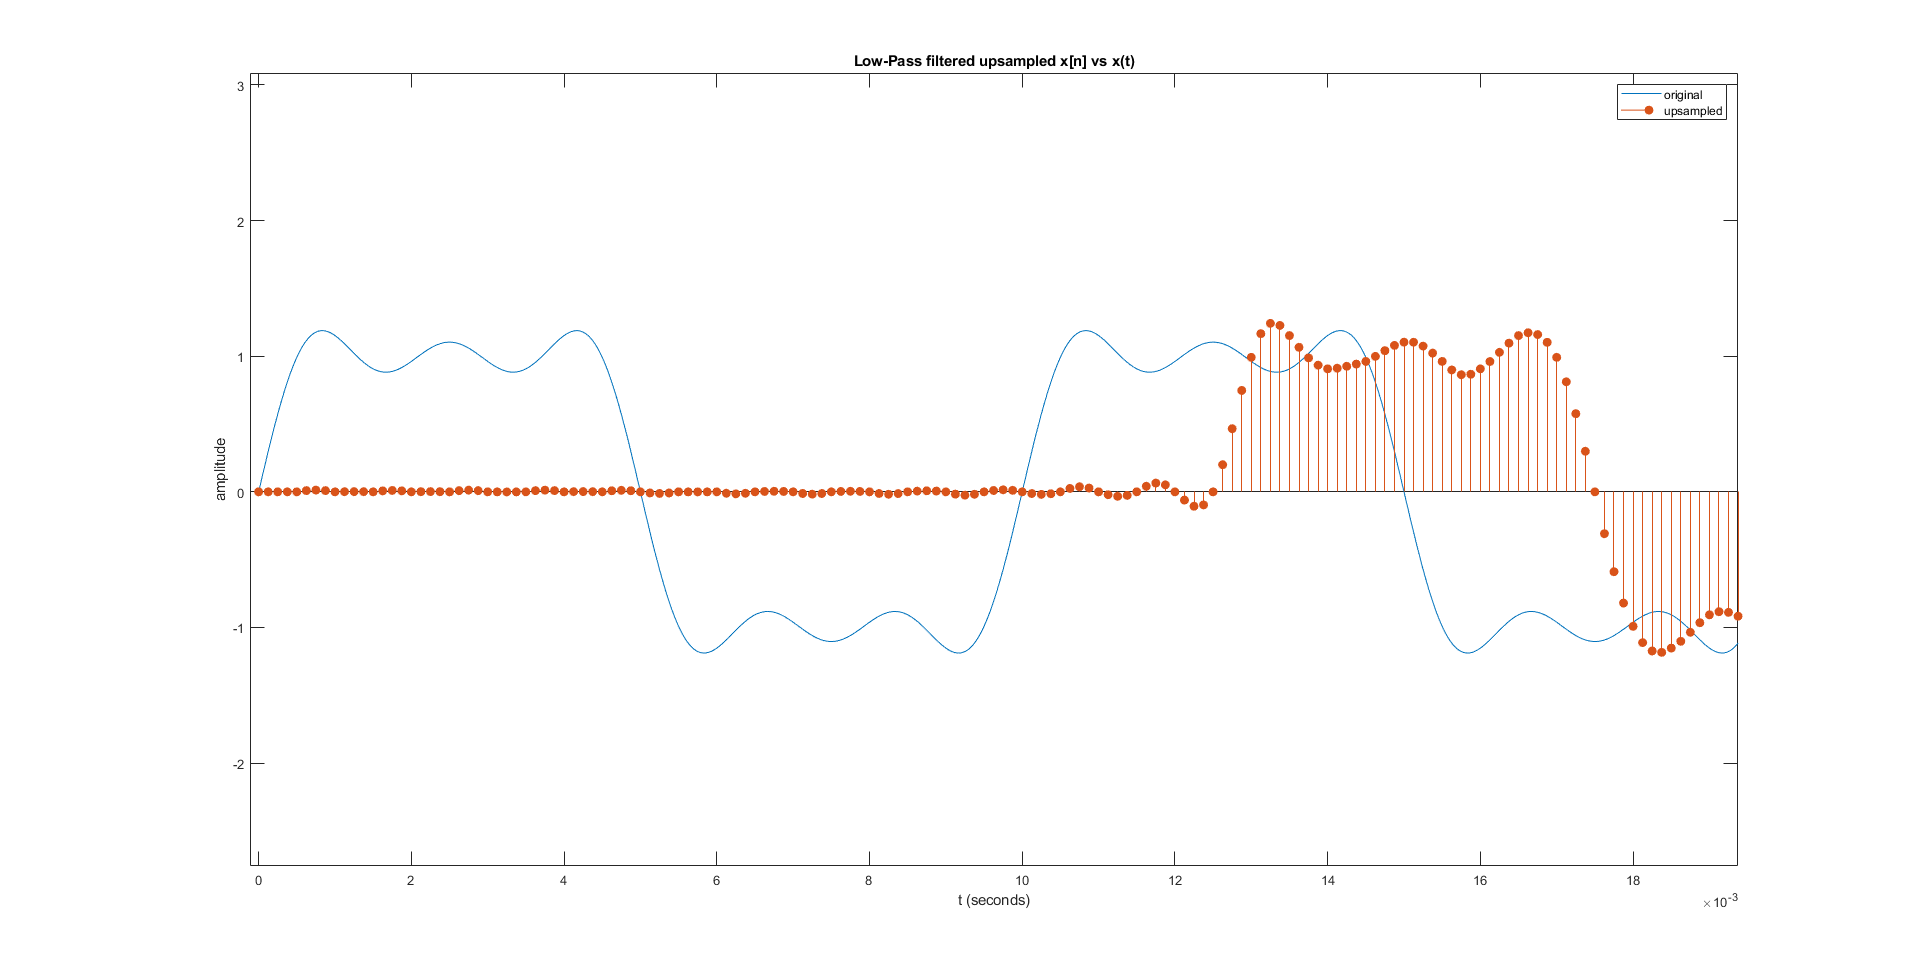
\includegraphics[width=0.8\textwidth]{fig6}
	\caption{Introduced delay}
\end{figure}

The previously shown figure focused on 30ms - 40ms of the signal. This is due to what figure 6 shows above; the induced filtering delay and warping at the beginning of the sequence.
%----------------------------------------------------------------------------------------
%	APPENDIX
%----------------------------------------------------------------------------------------
\newpage
\section*{Appendix}
\lstinputlisting[language=Matlab]{lab5.m}
\end{document}
